\documentclass[iop]{emulateapj}
% \documentclass[preprint]{aastex}
% \documentclass[12pt, onecolumn]{emulateapj}
% \documentstyle[aas2pp4,natbib209]{article}

\usepackage{tikz}
\usepackage{natbib}
\usepackage{amsmath}

\usetikzlibrary{shapes.geometric, arrows}
\usetikzlibrary{fit}

\tikzstyle{hyper} = [circle, text centered, draw=black]
\tikzstyle{param} = [circle, text centered, draw=black]
\tikzstyle{data} = [circle, text centered, draw=black, line width=2pt]
\tikzstyle{arrow} = [thick,->,>=stealth]

\newcommand{\myemail}{aimalz@nyu.edu}
\newcommand{\textul}{\underline}
\newcommand{\chippr}{\texttt{CHIPPR} }

\shorttitle{How to obtain the redshift distribution from probabilistic redshift estimates}
\shortauthors{Malz, et al.}

\begin{document}

\title{How to obtain the redshift distribution from probabilistic redshift estimates}

\author{Alex Malz\altaffilmark{1}, David W. Hogg\altaffilmark{1,2,3,4}, Phil Marshall\altaffilmark{5}, \& Others}
\email{aimalz@nyu.edu}

\altaffiltext{1}{Center for Cosmology and Particle Physics, Department of Physics,
  New York University, 726 Broadway, 9th floor, New York, NY 10003, USA}
\altaffiltext{2}{Simons Center for Computational Astrophysics, 162 Fifth Avenue, 7th floor, New York, NY 10010, USA}
\altaffiltext{3}{Center for Data Science, New York University, 60 Fifth Avenue, 7th floor, New York, NY 10003, USA}
\altaffiltext{4}{Max-Planck-Institut f\"ur Astronomie, K\"onigstuhl 17, D-69117 Heidelberg, Germany}
\altaffiltext{5}{[SLAC]}

\begin{abstract}
The redshift distribution $n(z)$ is a crucial ingredient for weak lensing cosmology.  Spectroscopically confirmed redshifts for the dim and numerous galaxies observed by weak lensing surveys are expected to be inaccessible, making photometric redshifts (photo-$z$s) the next best alternative.  Because of the nontrivial inference involved in their determination, photo-$z$ point estimates are being superseded by photo-$z$ probability distribution functions (PDFs).  However, analytic methods for utilizing these new data products in cosmological inference are still evolving.  This paper presents a novel approach to estimating the posterior distribution over $n(z)$ from a survey of galaxy photo-$z$ PDFs based upon a probabilistic graphical model of hierarchical inference.  We present the Cosmological Hierarchical Inference with Probabilistic Photometric Redshifts (\chippr) code implementing this technique, as well as its validation on mock data and testing on the \texttt{Buzzard} simulations.  \chippr yields a more accurate characterization of $n(z)$ containing information beyond the best-fit estimator produced by traditional procedures.  The publicly available code is easily extensible to other one-point statistics that depend on redshift.

\end{abstract}

\keywords{catalogs --- cosmology: cosmological parameters --- galaxies: statistics --- gravitational lensing: weak --- methods: analytical --- methods: data analysis --- methods: statistical --- techniques: photometric}

\section{Introduction}
\label{sec:introduction}

After a brief literature review addressing how photo-$z$ PDFs are currently used in cosmology, this paper aims to answer the following questions:

\begin{itemize}
	\item Why should we question existing methods?
	\item How can we improve the effectiveness of using photo-$z$ PDFs in inference?
	\item How does the result of \chippr compare to established estimators in terms of the accuracy of $n(z)$?
	\item How significant is the effect of the discrepancy between $n(z)$ estimators on cosmological constraints?
\end{itemize}

\section{Method}
\label{sec:method}

This paper presents a mathematically consistent method for obtaining the posterior probability distribution over the redshift distribution $n(z)$ using a catalog of photo-$z$ PDFs.  We start by introducing some nomenclature, definitions, and symbols that will be used throughout Secs. \ref{sec:model}, \ref{sec:others}, and \ref{sec:implementation}.

We shall say the parameters comprising $\vec{\phi}$ define the redshift distribution under some functional form about which this method is agnostic, so long as the functional form evaluated with some true values of the parameters accurately describes the true $n(z)$.  Since the redshift distribution is itself a probability distribution, it may be written as $p(z | \vec{\phi})$.

Before jumping into the details of the model, it is crucial to settle on an interpretation of what a photo-$z$ PDF actually is.  When a photo-$z$ PDF is reported, it is an object containing information about galaxy $i$'s redshift $z_{i}$ based on its photometric data $\vec{d}_{i}$, making a photo-$z$ PDF a \textit{posterior} probability distribution.  The data $\vec{d}_{i}$ may be fluxes, magnitudes, colors, or any combination thereof.  We assume that the redshifts of the galaxies are not related to the redshifts or photometry of other galaxies in the survey, i.e. they are \textit{independent}.

In addition to the data $\vec{d}_{i}$, the photo-$z$ PDF also contains information imparted by assumptions that went into the process by which the photo-$z$ was made.  Those assumptions are only relevant insomuch as they impose a preference on the redshift distribution. Thus, they can be reduced to a sort of prior on the distribution of redshifts, which can be parametrized under the chosen functional form by parameters $\vec{\phi}^{*}$.  The redshift distribution $p(z | \vec{\phi}^{*})$ associated with the parameters in $\vec{\phi}^{*}$ shall be called the interim prior because in many cases it was our best guess as to the true redshift distribution before observing any data.  For example, in template-based photo-$z$ PDF methods, the interim prior is a linear combination of the redshift distributions of the classes of templates based on previous observations.  (In training-based photo-$z$ PDF methods, the interim prior is related to the redshift distribution of the training set and thus may not be shared among all galaxies for which photo-$z$ PDFs are produced; however, in this work, we will assume that it is shared among all galaxies in a survey.)  Because the choice of parameters $\vec{\phi}^{*}$ is not causally connected to the data or the true redshift distribution but nonetheless contributes to the photo-$z$ PDF, we call it an \textit{interim prior}.  

A photo-$z$ PDF is then an \textit{interim posterior} probability distribution of the redshift of a galaxy given its observed photometric data and the interim prior: $p(z_{i} | \vec{d}_{i}, \vec{\phi}^{*})$.  We would like to learn about $p(z | \vec{\phi})$ from a catalog of photo-$z$ interim posteriors.

\subsection{Model}
\label{sec:model}

We present the two attributes of a probabilistic graphical model (PGM) for the redshift distribution $n(z)$: the directed acyclic graph (DAG) and its mathematical interpretation in terms of Bayesian hierarchical inference.  

The fundamental assumption underlying the concept of photo-$z$ estimation is that each galaxy $i$ has some observed photometric data $\vec{d}_{i}$ (fluxes, magnitudes, or colors) that is drawn from a function of its redshift $z_{i}$, which is a parameter in this model.  This function constitutes a forward model for the observations.  The redshifts $\{z_{i}\}$ for all galaxies in a survey are random draws from the redshift distribution, whose parameters  $\vec{\phi}$ under a chosen functional form are called \textit{hyperparameters} because they are shared among all $N$ galaxies in the survey.  Fig. \ref{fig:pgm} illustrates these relationships.  PGMs of this structure are \textit{hierarchical} in that, though the data are only directly influenced by their redshift parameters, we can still use them to infer something about the global hyperparameters by way of a higher level in the graph.

\begin{figure}
	\begin{center}
		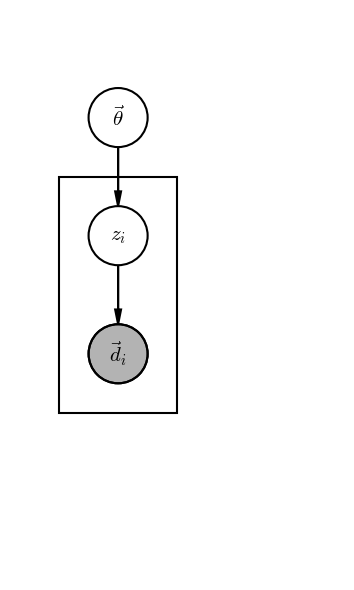
\includegraphics[width=0.5\textwidth]{pgm.png}
		\caption{This directed acyclic graph corresponds to a probabilistic graphical model for a Bayesian hierarchical inference of $p(\vec{\phi}|\{\vec{d}_{i}\})$.  In this graph, all random variables are shown in circles, with observed random variables shown in shaded circles.  Relationships between variables are indicated by arrows from parameters to the variables distributed according to functions of them.  The box indicates that there are a number of copies of the relationships between boxed parameters, each independent of all others.  The hyperparameters comprising $\vec{\phi}$, which define $n(z)$, are at the top.  Independently drawn from a function of the hyperparameters $\vec{\phi}$ are galaxy redshifts $\{z_{i}\}$ below.  The observed galaxy photometry $\{\vec{d}_{i}\}$, shown in shaded circles, is determined by the redshifts above.}
	\label{fig:pgm}
	\end{center}
\end{figure}

% It would be easy to estimate $\vec{\phi}$ given $\{z_{i}\}_{N}$, however, what we actually have is photometric data $\{\vec{d}_{i}\}_{N}$ which we used to derive photo-$z$ PDFs.  Because a photo-$z$ PDF is a probability distribution conditioned on the photometric data, it must be interpreted as a posterior probability distribution.  

% In addition to the data, the posterior probability distribution is conditioned on other information about how it was made, which is in general specific to the method that produced it.  This information only influences the posterior by its implicit distribution over redshifts, which we call the interim prior over redshift.  The interim prior, like the redshift distribution we wish to infer, has some functional form with some parameters, but since the redshift distribution and interim prior need not share the same parametrization, we will use $\vec{\alpha}$ to represent the parameters for the interim prior.  Thus, the posterior probability that is often oversimplified as "$p(z_{i})$" is really the interim posterior probability $p(z_{i} | \vec{d}_{i}, \vec{\alpha})$.  Note that we will assume that all galaxies whose photo-$z$ interim posteriors are derived by a single method share the same interim prior $p(z | \vec{\alpha})$; depending on the method, this may not always be true.

The DAG of Fig. \ref{fig:pgm} translates directly into a mathematical expression for the posterior distribution $p(\vec{\phi} | \{\vec{d}_{i}\})$ of the hyperparameters given the entire set of interim posteriors $\{p(z_{i} | \vec{d}_{i}, \vec{\phi}^{*})\}$ by way of the following derivation.  From this point forward, we will use log probabilities.

According to Bayes' rule, the posterior distribution of interest is
\begin{align}
\log p(\vec{\phi} | \{\vec{d}_{i}\}) &\propto \log p(\{\vec{d}_{i}\} | \vec{\phi}) + \log p(\vec{\phi}),
\end{align}
where $p(\vec{\phi})$ is the \textit{hyperprior} probability distribution over possible values of the hyperparameters.  The hyperprior is a choice made by those performing the inference and is not to be confused with the interim prior parameters that influence the photo-$z$ PDF data product.

Focusing on the likelihood term $p(\{\vec{d}_{i}\} | \vec{\phi})$, we employ the power of the hierarchical model through \textit{marginalization} of the unobserved redshift parameters by integrating over them to obtain 
\begin{align}
\log[p(\{\vec{d}_{i}\} | \vec{\phi})] &= \log[\int\exp[\log[p(\{\vec{d}_{i}\} | \{z_{i}\})]\\
& + \log[p(\{z_{i}\} | \vec{\phi})]]\ d\{z_{i}\}].
\end{align}


Given a catalog of photo-$z$ interim posteriors $\{p(z_{i} | \vec{d}_{i}, \vec{\alpha})\}$

To make use of the photo-$z$ interim priors, it is absolutely essential that $\vec{\alpha}$ be known.  

This framework entails a number of choices and assumptions that must be addressed explicitly.

\begin{enumerate}
	\item The chosen functional form with parameters $\vec{\phi}$ must actually be able to describe the true redshift distribution.
	\item The photometric data and redshift for each galaxy is independent of the photometric data and redshifts of all other galaxies.
	\item There is one interim prior with parameters $\vec{\phi}^{*}$ shared among all galaxies in the survey.
	\item We must choose a hyperprior probability distribution $p(\vec{\phi})$ over the hyperparameters.
	\item While we advocate for the approach of hierarchical inference, the probabilistic graphical model presented here is not the only one that could be proposed.
\end{enumerate}

\subsection{Alternative Approaches}
\label{sec:others}

It is useful to translate some popular existing methods for deriving $n(z)$ from photo-$z$ PDFs into the mathematical framework of Sec. \ref{sec:model}.

\subsection{Implementation}
\label{sec:implementation}

The publicly available \chippr code implements the probabilistic graphical model presented in Sec. \ref{sec:model}.  

In addition to the choices and assumptions underlying the probabilistic graphical model, the implementation of \chippr makes choices and assumptions of its own.

\begin{enumerate}
	\item \chippr currently only accepts photo-$z$ PDFs and produces $n(z)$ samples of a single format, that of the piecewise constant parametrization, also referred to as a binned histogram parametrization and a sum of top hat functions.
\end{enumerate}

\section{Validation on Simple Mock Data}
\label{sec:validation}

We demonstrate the superiority of \chippr over alternative approaches in a number of compelling test cases on mock data.  Each experiment is characterized by a single change to a fiducial case in order to isolate the influence of systematic effects known to be relevant to photo-$z$ estimation and propagation in analysis.  

\subsection{Mock Data \& Metrics}
\label{sec:validintro}

The mock data in these tests consists of photo-$z$ interim posteriors rather than photometric data because the various existing methods for deriving photo-$z$ interim posteriors do not in general yield results that are consistent with one another, indicating that their systematics are not well-understood.  Because the mock data is independent of any choice of photo-$z$ PDF production method, we not only ensure that our photo-$z$ interim priors are perfectly understood but also deter readers from assuming that \chippr has any preference over the method by which photo-$z$ interim posteriors are derived from photometric data.

\subsubsection{Mock Data}
\label{sec:mockdata}

The mock data used here are produced by the following steps.

\begin{enumerate}
	\item \label{itm:true} Choose a true $n(z)$ that is a continuous function with known parameters $\vec{\theta}$.
	\item \label{itm:sample} Sample the true $n(z)$ to create a catalog of $N$ true redshifts $z_{i}$.
	\item \label{itm:scatter} Choose a true intrinsic scatter $\sigma$, and sample Gaussians $p(z'_{i} | z_{i}, \sigma) = \mathcal{N}(z_{i}, \sigma)$ to get "observed" redshifts $z'_{i}$ defining Gaussian likelihoods $p(\vec{d}_{i} | z'_{i}, \sigma) = \mathcal{N}(z'_{i}, \sigma)$.
	\item \label{itm:interim} Choose a parametrization and the parameters $\vec{\phi}^{*}$ of the interim prior.
	\item \label{itm:posterior} Create interim posteriors $p(z_{i} | \vec{d}_{i}, \vec{\phi}^{*}) = p(\vec{d}_{i} | z_{i})\ p(z_{i} | \vec{\phi}^{*})$ in this parametrization.
\end{enumerate}

In all of the following validation tests, we use $10$ bins and $N = 10,000$ galaxies.  In Secs. \ref{sec:truth} and \ref{sec:likelihoods}, we use a flat interim prior.  This method for deriving mock data is referred to as the fiducial case, and variations on it will refer directly to the steps that are altered.

\subsubsection{$n(z)$ Accuracy Metric}
\label{sec:accuracy}

The Kullback-Leibler divergence is our primary measure of the accuracy of estimators of $n(z)$ in cases of mock data with known true redshifts.

\textbf{Review precision and bias from \texttt{kld.ipynb} and interpret in terms of a \% difference.}

\subsection{Underlying $n(z)$ Effects}
\label{sec:truth}

Existing $n(z)$ estimators are systematically smoother than the true $n(z)$.  Here we show that the traditional estimators perform better when the true $n(z)$ is weakly featured than when the true $n(z)$ is strongly featured by experimenting with Step \ref{itm:true} of Sec. \ref{sec:mockdata}.  The implication of this issue is quite serious; the consistently smooth, unimodal $n(z)$ estimates appearing in the literature could result from much more featured true redshift distributions, and there would be no way to catch this error without using a fully probabilistic method.

\subsubsection{Featureless $n(z)$}
\label{sec:smooth}

In this test, we choose a weakly featured true $n(z)$ of Fig. \ref{fig:smooth} with a smooth, unimodal shape, based on the interim prior used for the SDSS DR8 photo-$z$ PDFs.  [check and include citation!]

\begin{figure}
	\begin{center}
		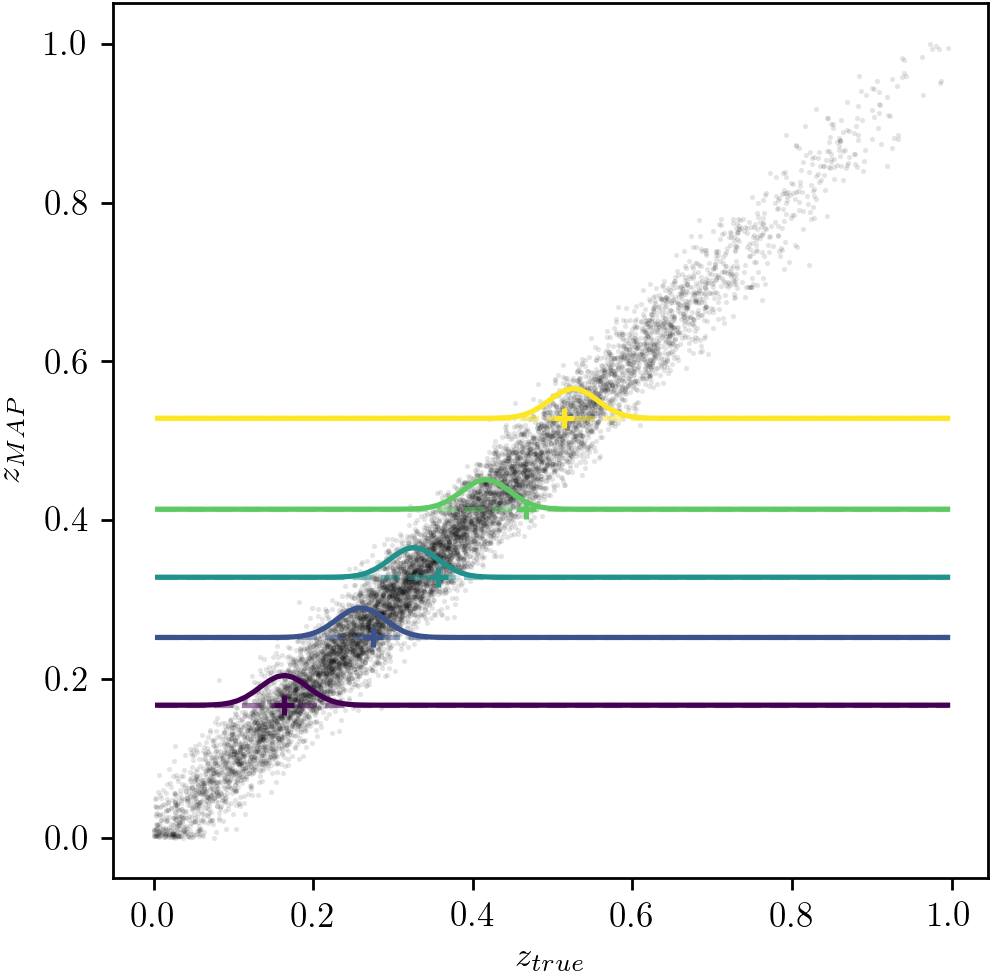
\includegraphics[width=0.5\textwidth]{fig/smooth_truth/scatter.png}\\
		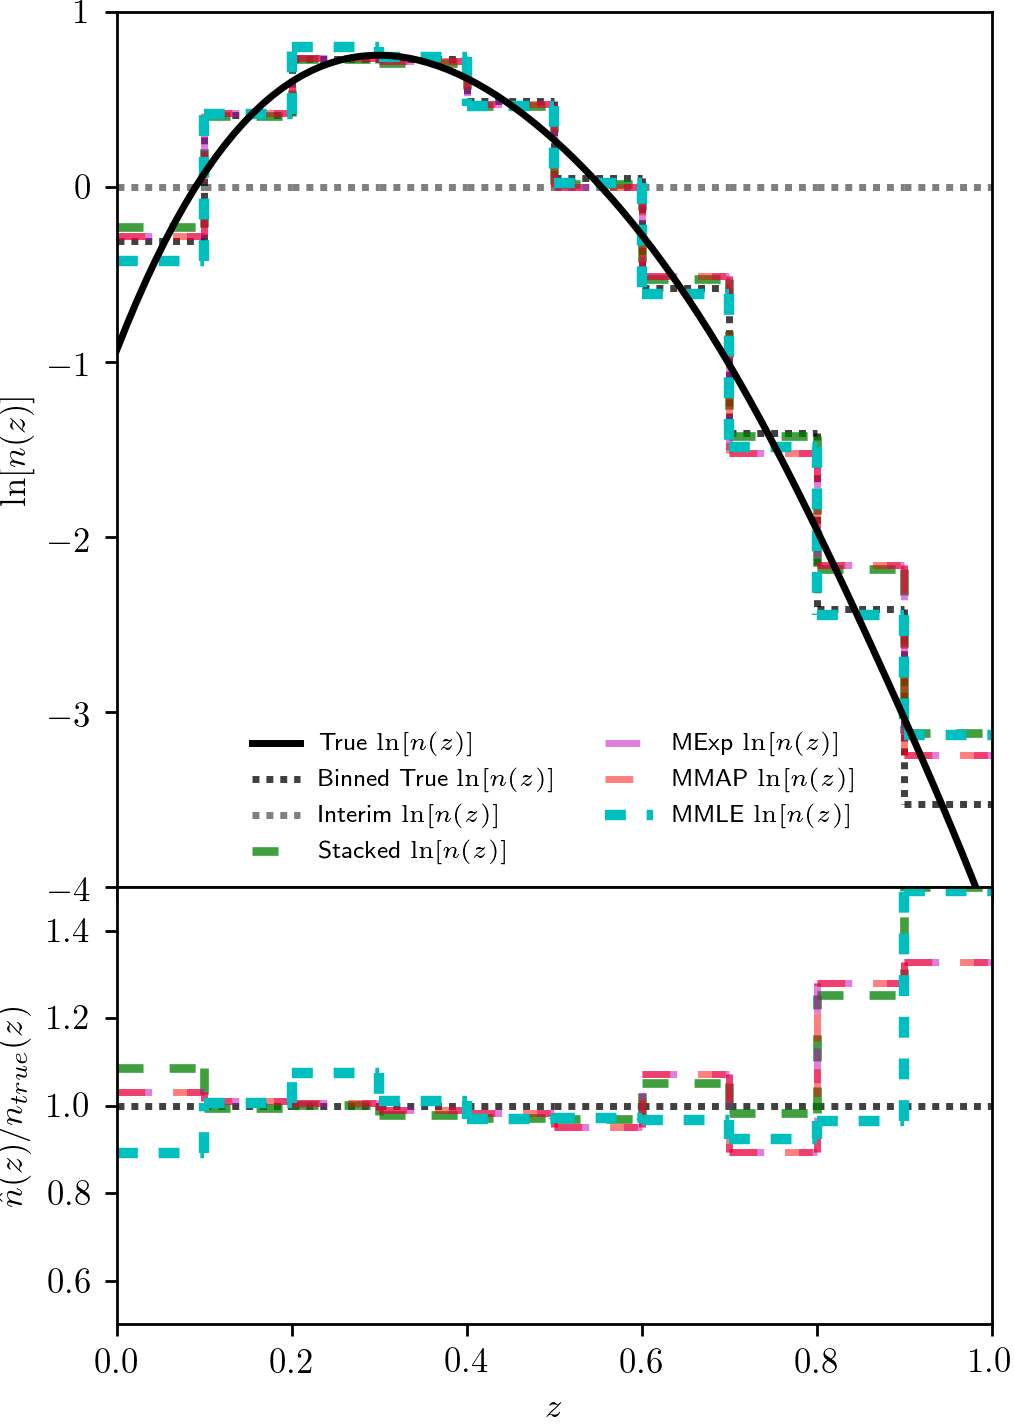
\includegraphics[width=0.5\textwidth]{fig/smooth_truth/estimators.png}	
		\caption{All estimators perform well when the true $n(z)$ is well behaved, exhibiting significant deviation only when $n(z)$ is very small, as the sample size of true redshifts in that range will be small.  Top panel: The traditional MAP reduction of a photo-$z$ PDF against the true redshifts with a few rescaled photo-$z$ interim posteriors are overplotted in solid lines, with a dotted line indicating zero probability.  Bottom panel: Various estimators of $\ln[n(z)]$, the interim prior, and the true $\ln[n(z)]$ as a continuous function and under a binned parametrization.}
		\label{fig:featured}
	\end{center}
\end{figure}

\subsubsection{Featured $n(z)$}
\label{sec:featured}

In this test, we choose the true $n(z)$ of Fig. \ref{fig:featured} with nontrivial structure.

\begin{figure}
	\begin{center}
		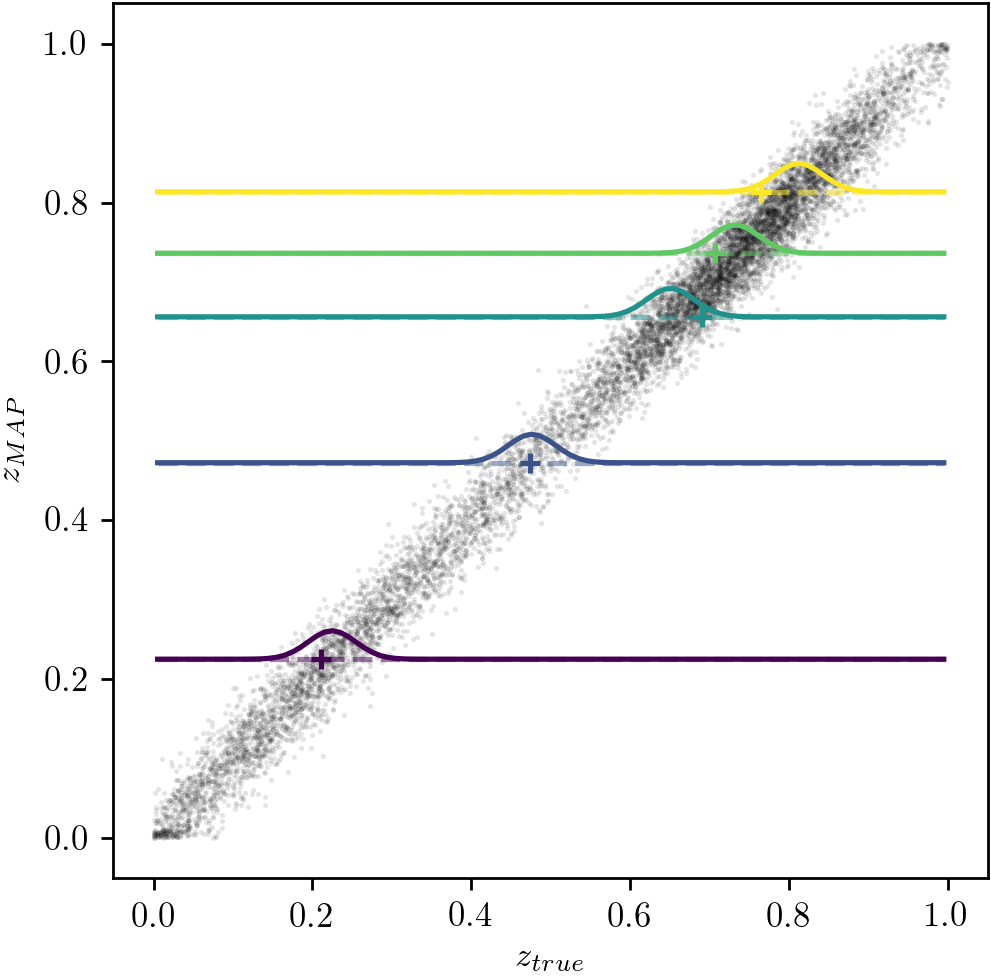
\includegraphics[width=0.5\textwidth]{fig/fiducial/scatter.png}\\
		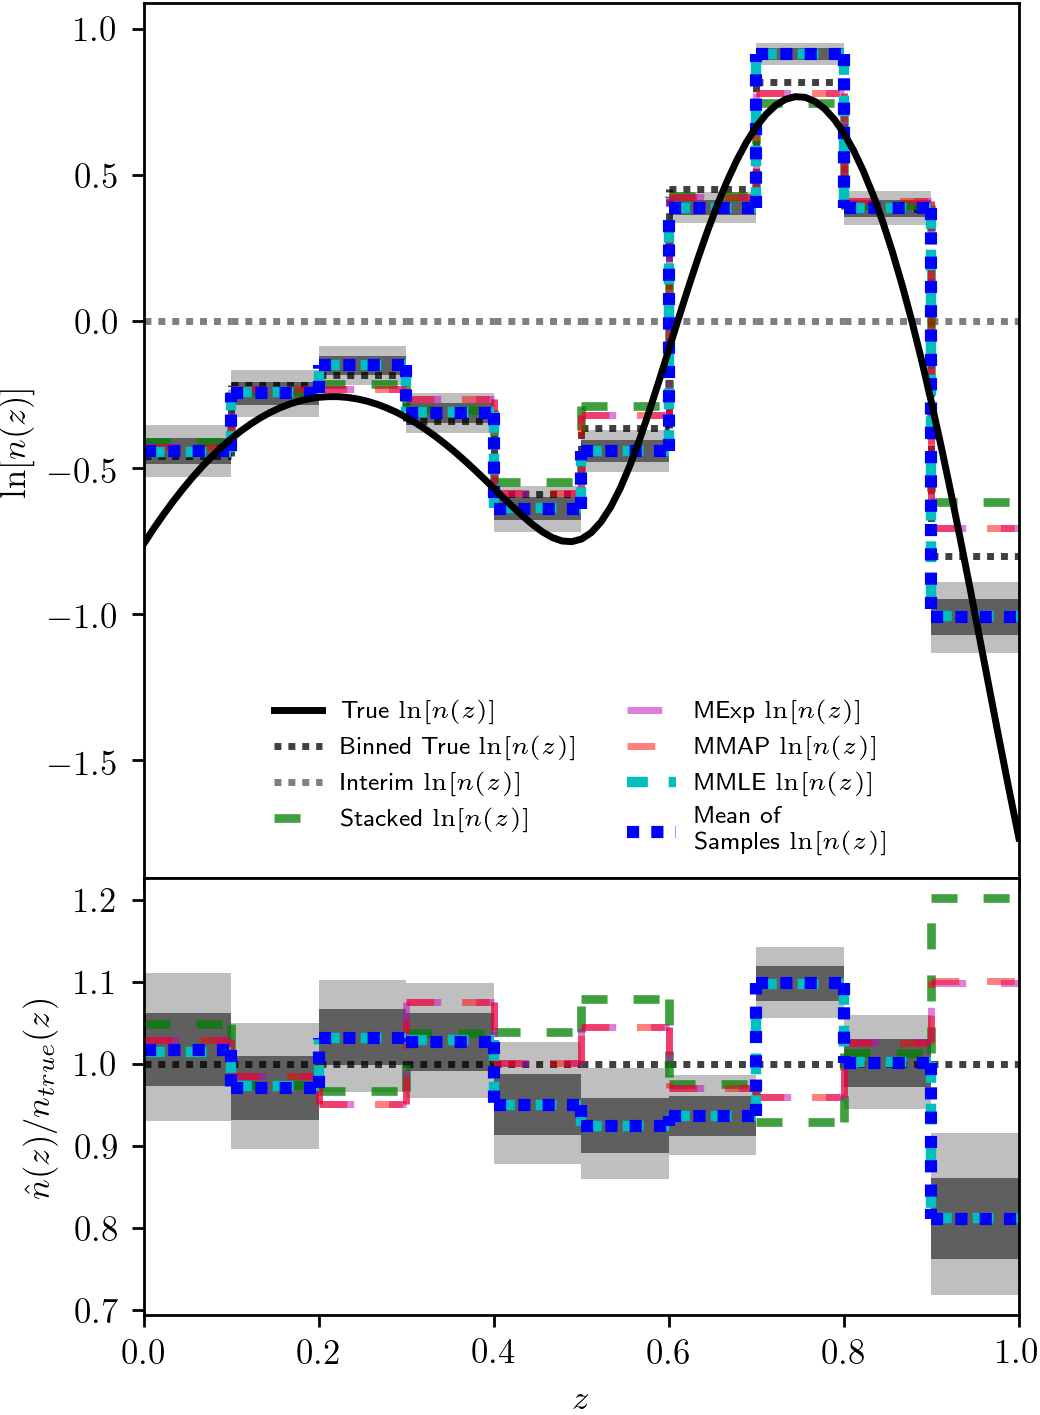
\includegraphics[width=0.5\textwidth]{fig/fiducial/estimators.png}		
		\caption{[This plot doesn't really show what I want because the intrinsic scatter is too low!  I used $\sigma=0.03$ because that's what has been quoted as what LSST, etc. needs, but that's not what comes out of photo-$z$ estimation methods before they impose aggressive cuts\dots]  Top panel: The traditional MAP reduction of a photo-$z$ PDF against the true redshifts with a few rescaled photo-$z$ interim posteriors are overplotted in solid lines, with a dotted line indicating zero probability.  Bottom panel: Various estimators of $\ln[n(z)]$, the interim prior, and the true $\ln[n(z)]$ as a continuous function and under a binned parametrization.}
		\label{fig:featured}
	\end{center}
\end{figure}

This featured true $n(z)$ will henceforth be referred to as the fiducial $n(z)$

\subsection{Emulated Data Quality Effects}
\label{sec:likelihoods}

In the following test cases, we vary the properties of the mock photo-$z$ likelihoods in an effort to emulate known systematics in photo-$z$ estimation.  These tests vary Step \ref{itm:scatter} of Sec. \ref{sec:mockdata}.

\subsubsection{Intrinsic Scatter}
\label{sec:intscat}

One major concern about photo-$z$s is the intrinsic scatter of point estimators, including those derived from photo-$z$ PDFs, that is observed to varying extents with every existing photo-$z$ algorithm and illustrated in Fig. \ref{fig:intscat}.  To emulate intrinsic scatter, we modify the fiducial case to simply broaden the single Gaussian component of the likelihood.  To enforce self-consistency, the mean is a random variable drawn from a Gaussian distribution with the newly increased variance.

\begin{figure}
	\begin{center}
		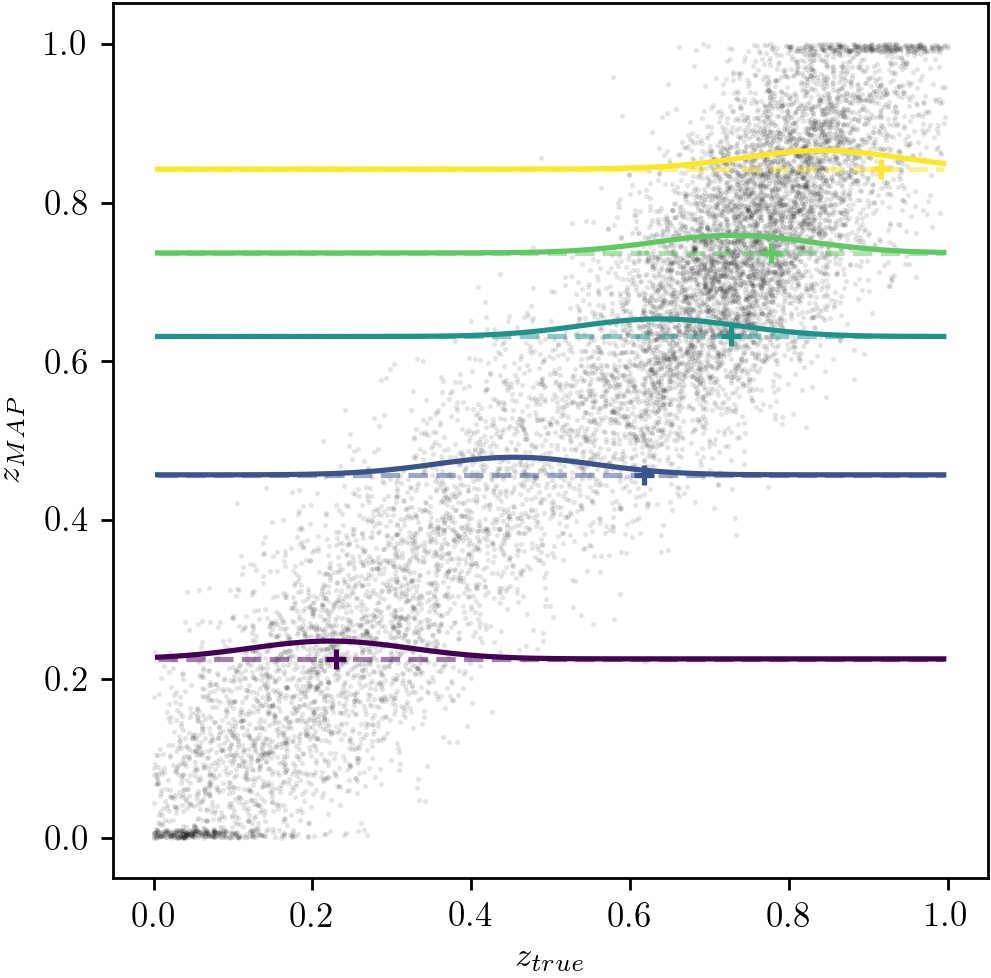
\includegraphics[width=0.5\textwidth]{fig/high_scatter/scatter.png}\\
		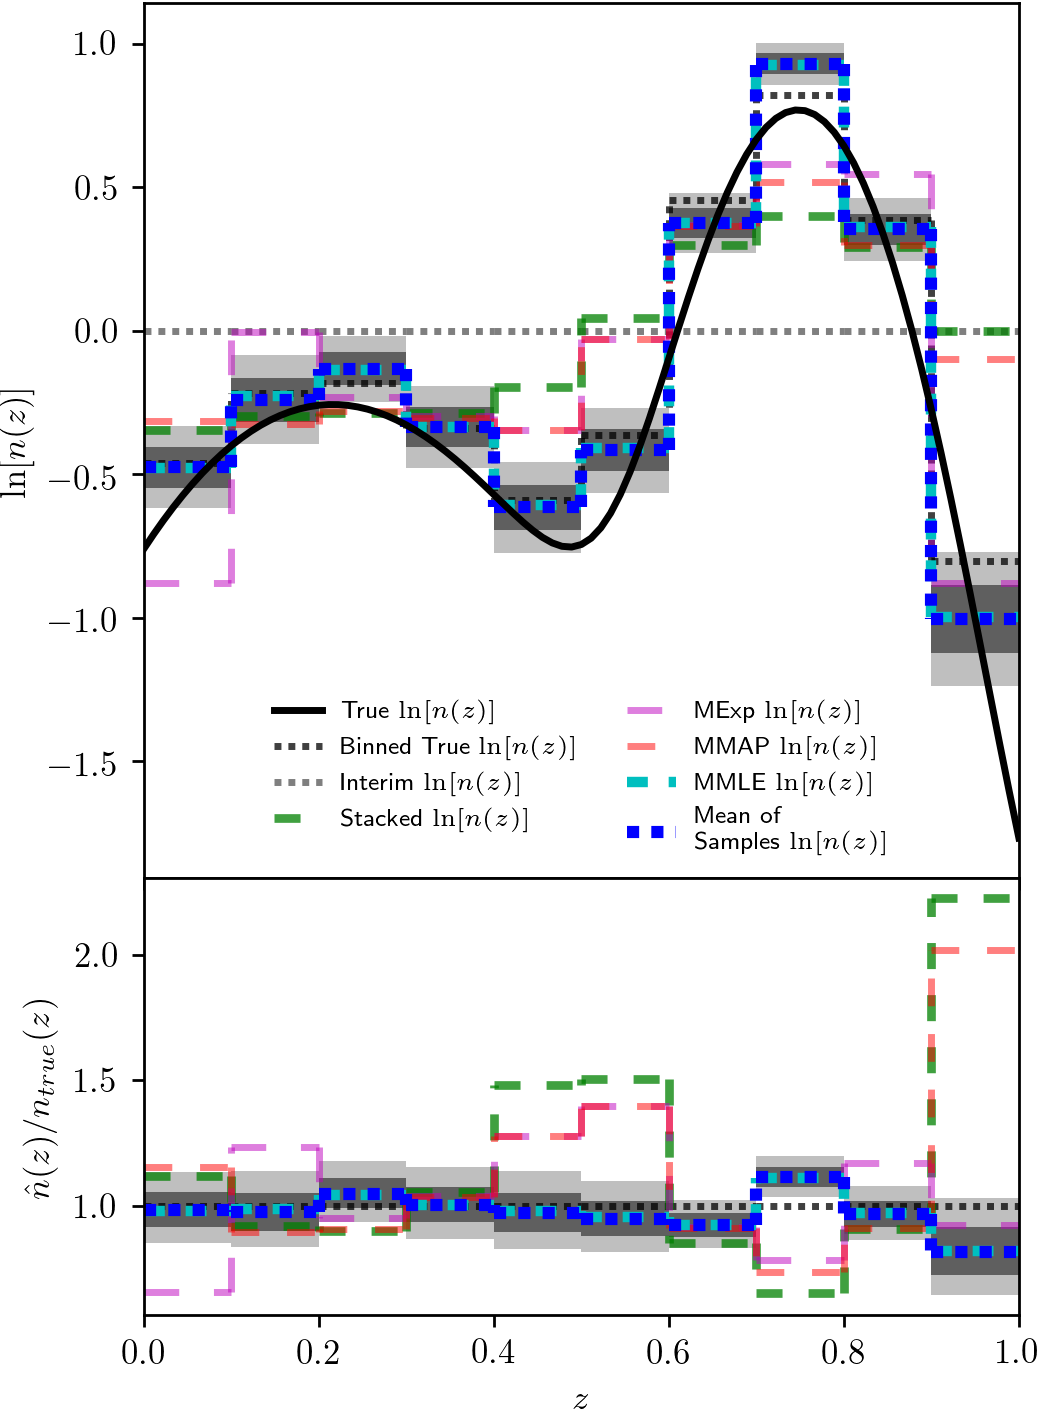
\includegraphics[width=0.5\textwidth]{fig/high_scatter/estimators.png}		
		\caption{As the intrinsic scatter increases, the discrepancy between estimators increases.  In particular, the stacked estimator and marginalized point estimators predict $\ln[n(z)]$ to be smoother than the truth, while the  [This would be a lot more compelling with more galaxies.  Also, the weird edge effects in the top panel are real, because the point estimator is the MAP, not the center of the Gaussian likelihood, and there's no requirement that the mean of the likelihood be within the true redshift range.]  Top panel: The traditional MAP reduction of a photo-$z$ PDF against the true redshifts with a few rescaled photo-$z$ interim posteriors are overplotted in solid lines, with a dotted line indicating zero probability.  Bottom panel: Various estimators of $\ln[n(z)]$, the interim prior, and the true $\ln[n(z)]$ as a continuous function and under a binned parametrization.}
		\label{fig:intscat}
	\end{center}
\end{figure}

To emulate intrinsic scatter, we modify the fiducial case to simply broaden the single Gaussian component of the likelihood.  To enforce self-consistency, the mean is a random variable drawn from a Gaussian distribution with the newly increased variance.

\subsubsection{Template-like Catastrophic Outliers}
\label{sec:tempcatout}

In addition to intrinsic scatter, photo-$z$ methods employing template fitting tend to produce catastrophic outliers that are distributed to be broad in $z_{spec}$ and narrow in $z_{phot}$, as in Fig. \ref{fig:tempcatout}.  The systematic behind these catastrophic outliers may be described as an attractor in the space of $z_{phot}$; some galaxies at a range of $z_{spec}$ map onto a single $z_{phot}$ (with some scatter) if their true SED does not have sufficiently strong features (as is the case for blue galaxies), leading galaxies of that SED type at many $z_{spec}$ to have similar colors.

\begin{figure}
	\begin{center}
		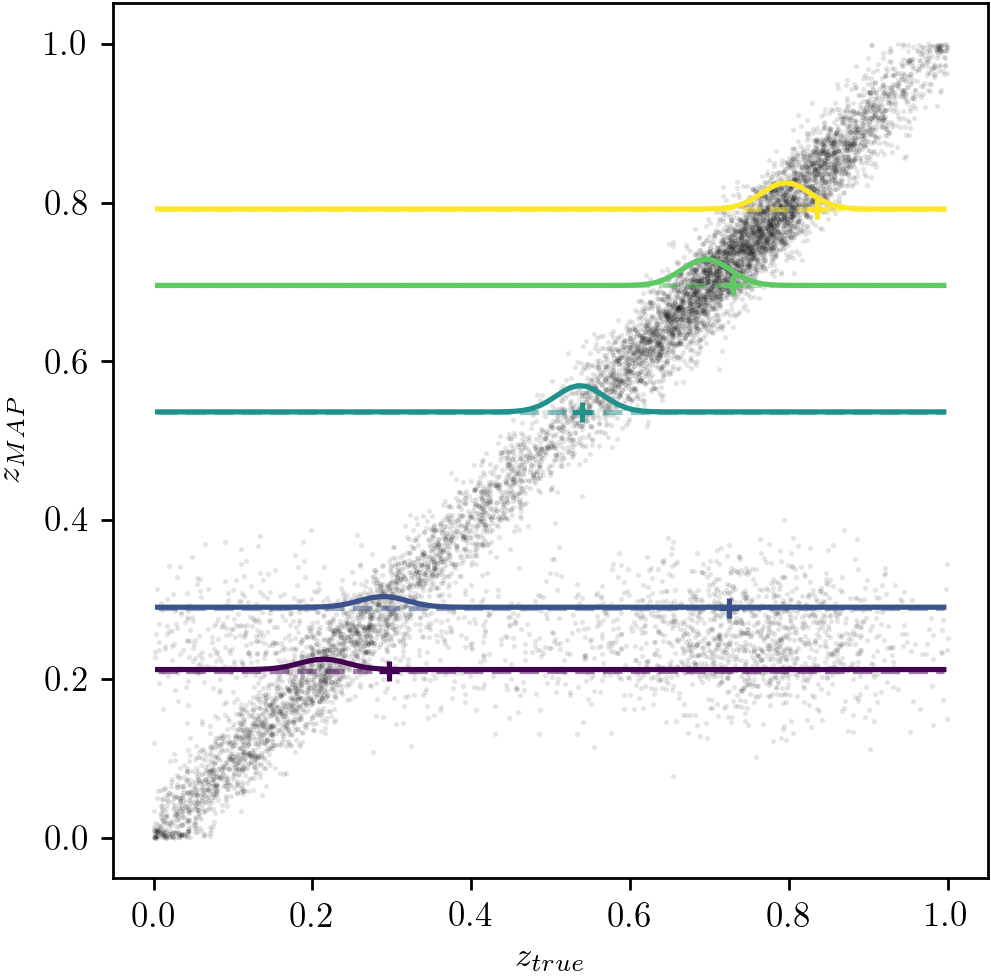
\includegraphics[width=0.5\textwidth]{fig/template_outliers/scatter.png}\\
		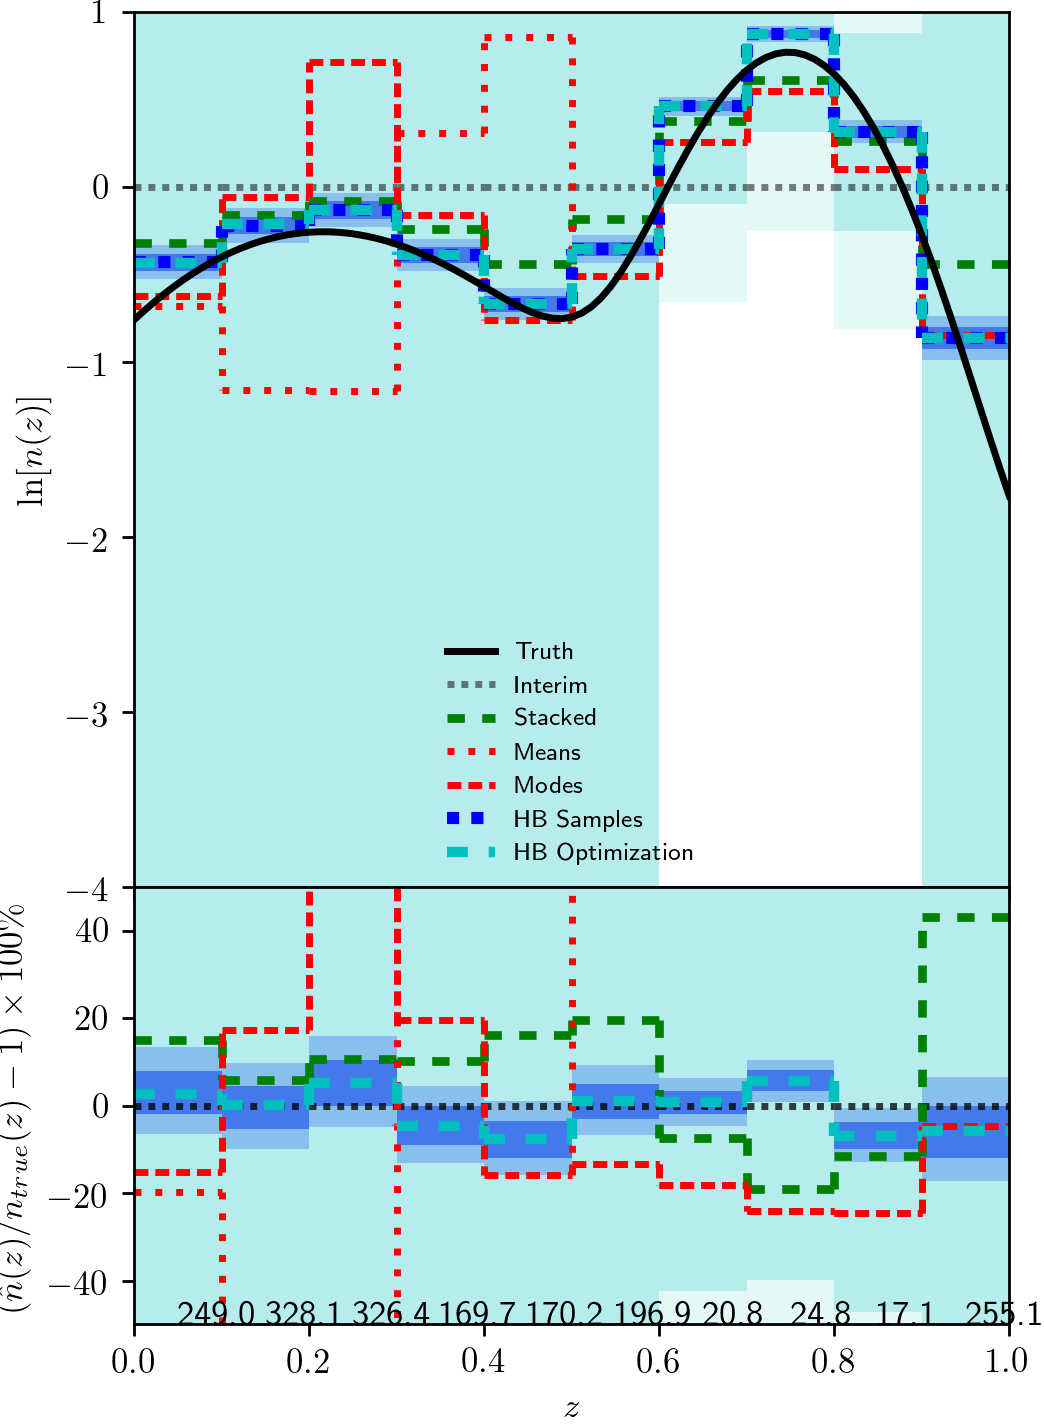
\includegraphics[width=0.5\textwidth]{fig/template_outliers/estimators.png}		
		\caption{Top panel: The traditional MAP reduction of a photo-$z$ PDF against the true redshifts with a few rescaled photo-$z$ interim posteriors are overplotted in solid lines, with a dotted line indicating zero probability.  Bottom panel: Various estimators of $\ln[n(z)]$, the interim prior, and the true $\ln[n(z)]$ as a continuous function and under a binned parametrization.}
		\label{fig:tempcatout}
	\end{center}
\end{figure}

\subsubsection{Training-like Catastrophic Outliers}
\label{sec:traincatout}

Data driven photo-$z$ methods tend to suffer from a different form of catastrophic outliers that are distributed to be narrow in $z_{spec}$ and broad in $z_{phot}$, as in Fig. \ref{fig:traincatout}.  The systematic behind these catastrophic outliers may be described as an attractor in the space of $z_{spec}$; some galaxies near a particular $z_{spec}$ map to a range of $z_{phot}$ if the training set galaxies at that $z_{spec}$ have inconsistent $z_{phot}$, as might occur if their SED's features fall between photometric filters.

\begin{figure}
	\begin{center}
		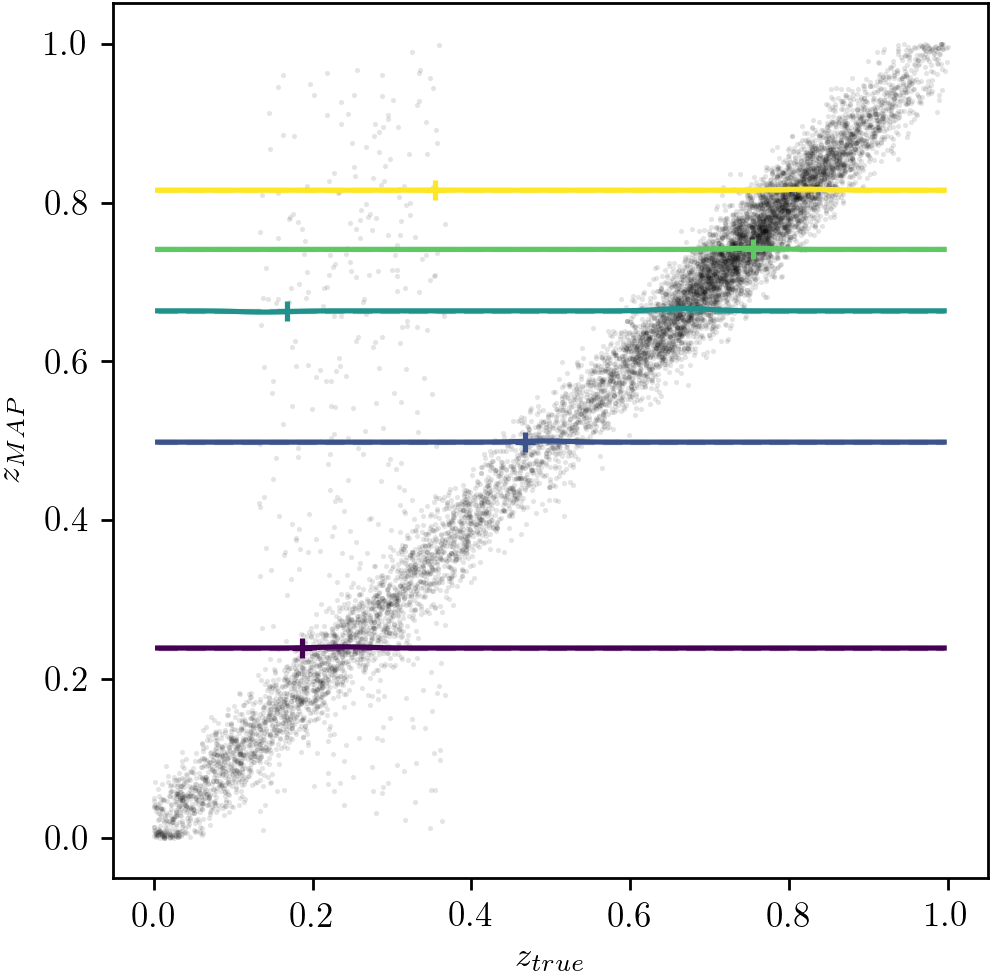
\includegraphics[width=0.5\textwidth]{fig/training_outliers/scatter.png}\\
		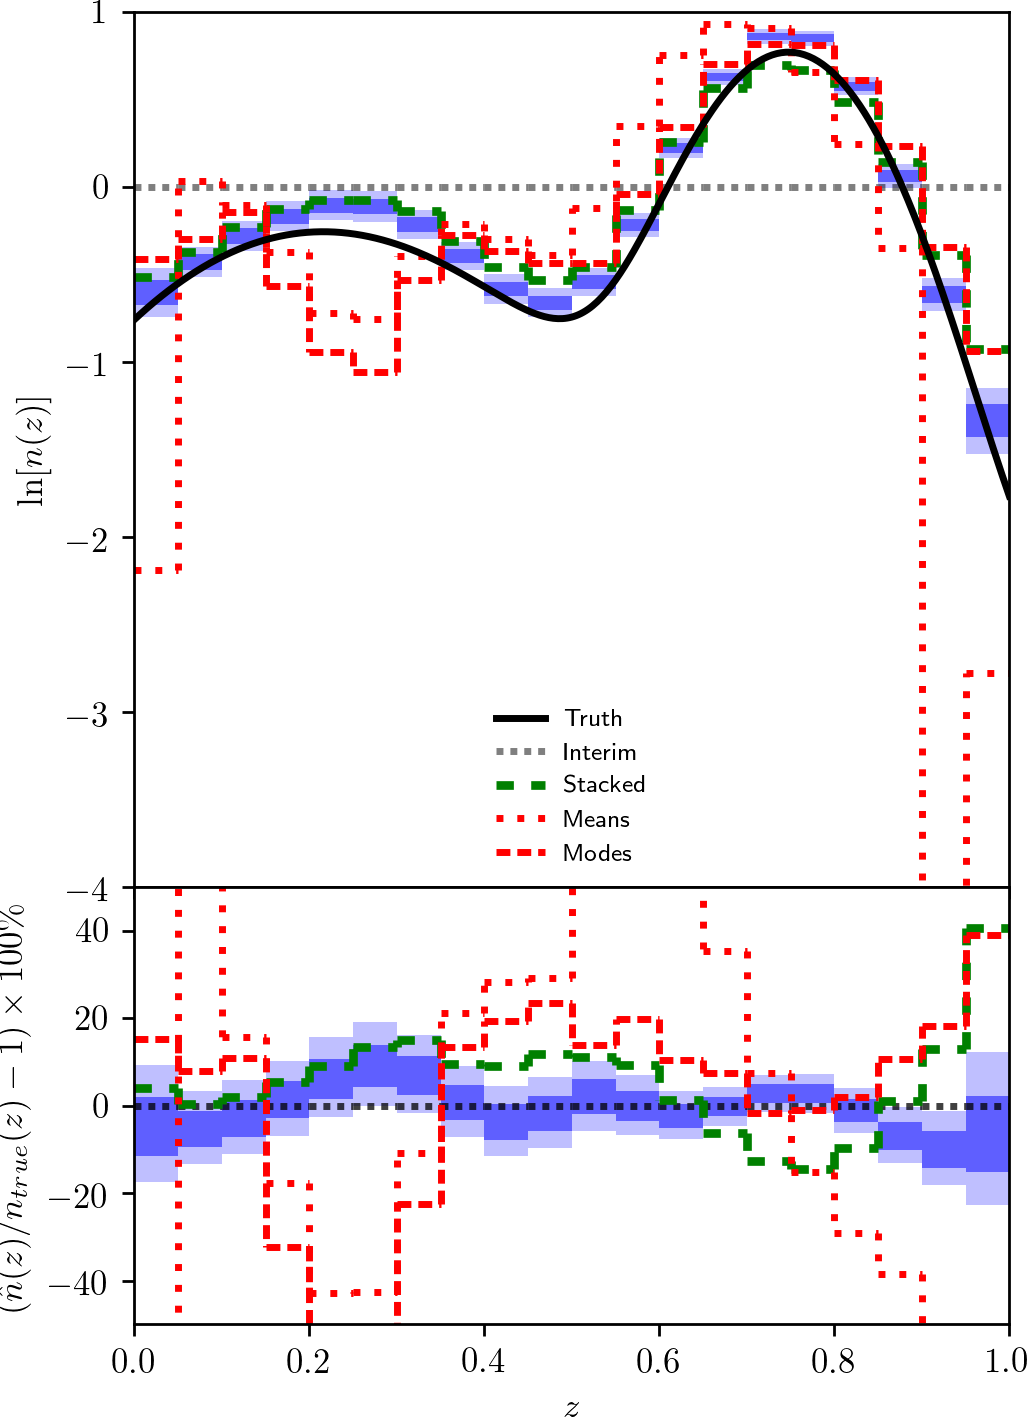
\includegraphics[width=0.5\textwidth]{fig/training_outliers/estimators.png}	
		\caption{[This has proven to be the most challenging test case to implement, and there's clearly still a bug in the function that makes the likelihoods.]}
		\label{fig:traincatout}
	\end{center}
\end{figure}

\subsection{Emulated Interim Prior Effects}
\label{sec:priors}

The interim prior encapsulates the the relationship between observed photometry and redshift information upon which a photo-$z$ estimate is based.  Interim priors are in general not identical to the true $n(z)$ we wish to estimate; if they were, we would not need any data!  For template fitting photo-$z$ methods, the interim prior is usually an input chosen by the researcher.  However, for machine learning methods, the interim prior is some function of the training set data that in many cases may be influenced by random numbers and is rarely output with the redshift estimates.  Interim priors for template fitting methods tend to have incomplete coverage in the space of true photometry, because they are limited by the choice of the library of SEDs.  Interim priors for machine learning methods tend to have incomplete coverage in the space of redshifts, because there are fewer galaxies with spectroscopically confirmed redshifts at high redshifts than low redshifts.

Existing $n(z)$ estimation routines will always produce a biased estimator when the interim prior is not equal to the true $n(z)$.  We demonstrate here that regardless of the appropriateness of the interim prior as an approximation to the true $n(z)$, \chippr is not affected by the choice of the interim prior so long as it has nontrivial coverage in the space of redshift.  These tests modify Step \ref{itm:interim} of Sec. \ref{sec:mockdata}.

\subsubsection{Template-like Interim Prior}
\label{sec:tempintpr}

An interim prior based on a template library may be a sum of smooth functions representing $n(z)$ for each SED type in the library.  Template libraries do not include every possible galaxy SED, and the $n(z)$ used for each SED type may not be accurate.  The interim prior shown in Fig. \ref{fig:tempintpr} is an emulation of an interim prior corresponding to a template library of this type.

\begin{figure}
	\begin{center}
		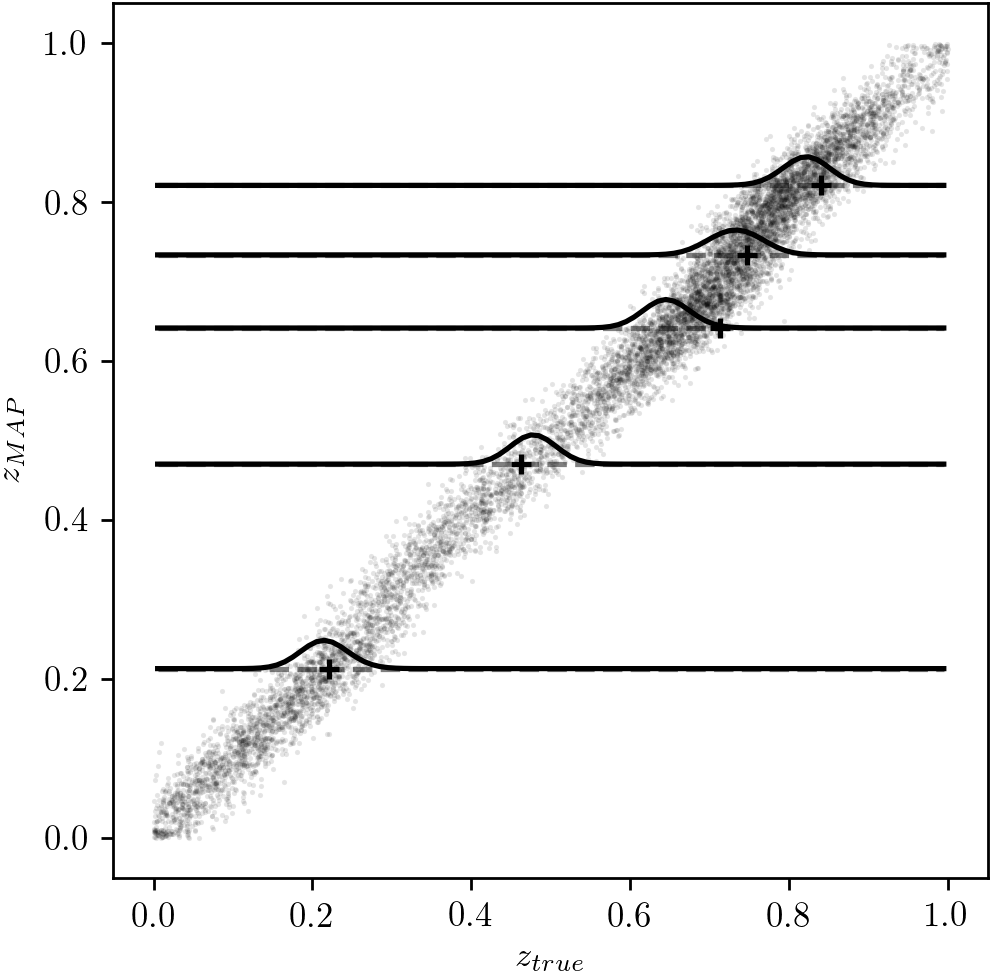
\includegraphics[width=0.5\textwidth]{fig/template_prior/scatter.png}\\
		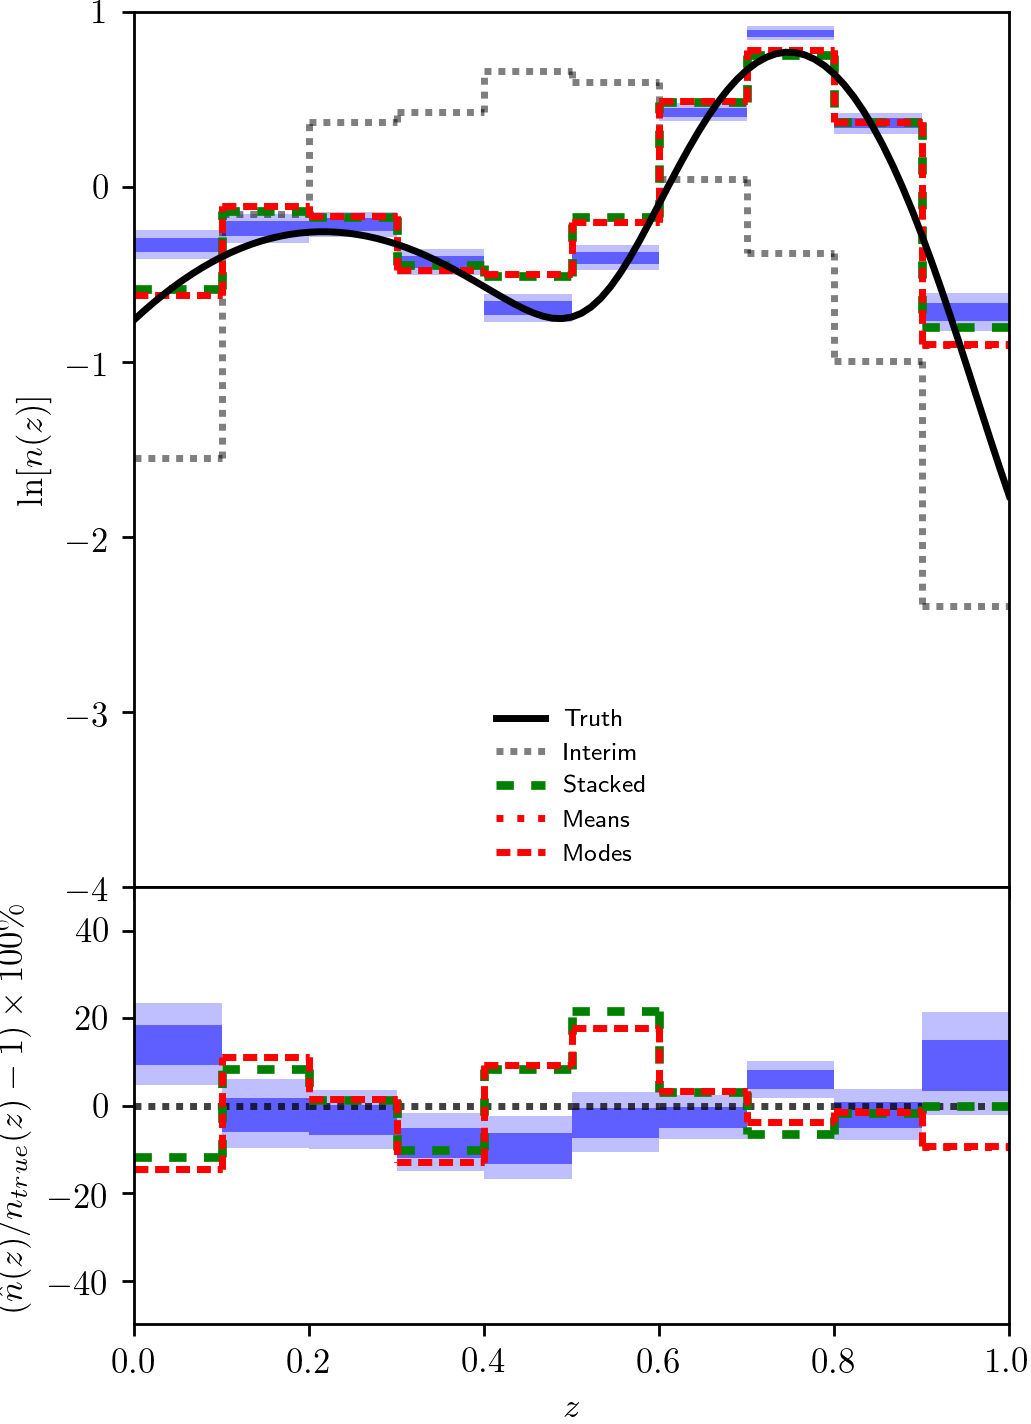
\includegraphics[width=0.5\textwidth]{fig/template_prior/estimators.png}	
		\caption{[The case of a multimodal interim prior was a very compelling test in the previous version but somehow isn't anymore.]}
		\label{fig:tempintpr}
	\end{center}
\end{figure}

\subsubsection{Training-like Interim Prior}
\label{sec:trainintpr}

An interim prior based on a training set may be biased toward low redshifts due to the dearth of distant galaxies with spectroscopic redshifts.  The interim prior shown in Fig. \ref{fig:trainintpr} is an emulation of an interim prior corresponding to a training set biased in this way.  We chose an interpolation of the interim prior used for the SDSS DR8 photo-$z$ PDFs.  

\begin{figure}
	\begin{center}
		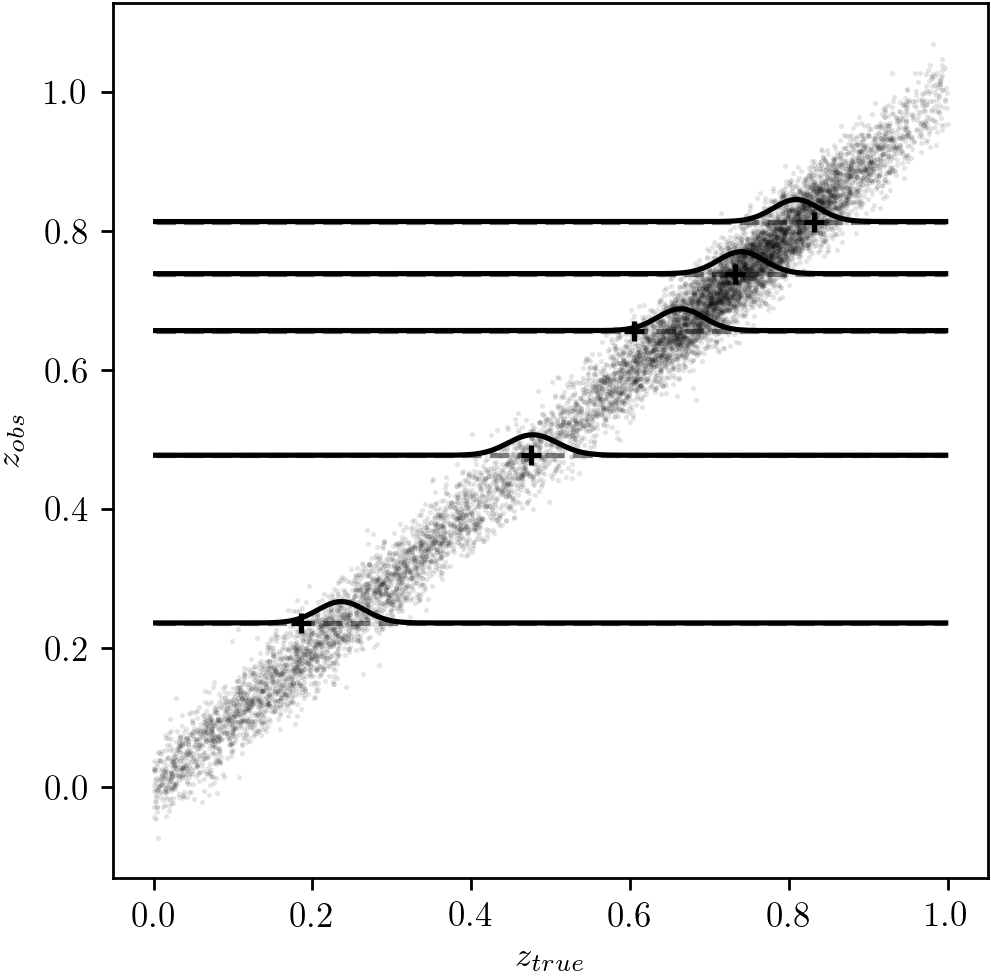
\includegraphics[width=0.5\textwidth]{fig/training_prior/scatter.png}\\
		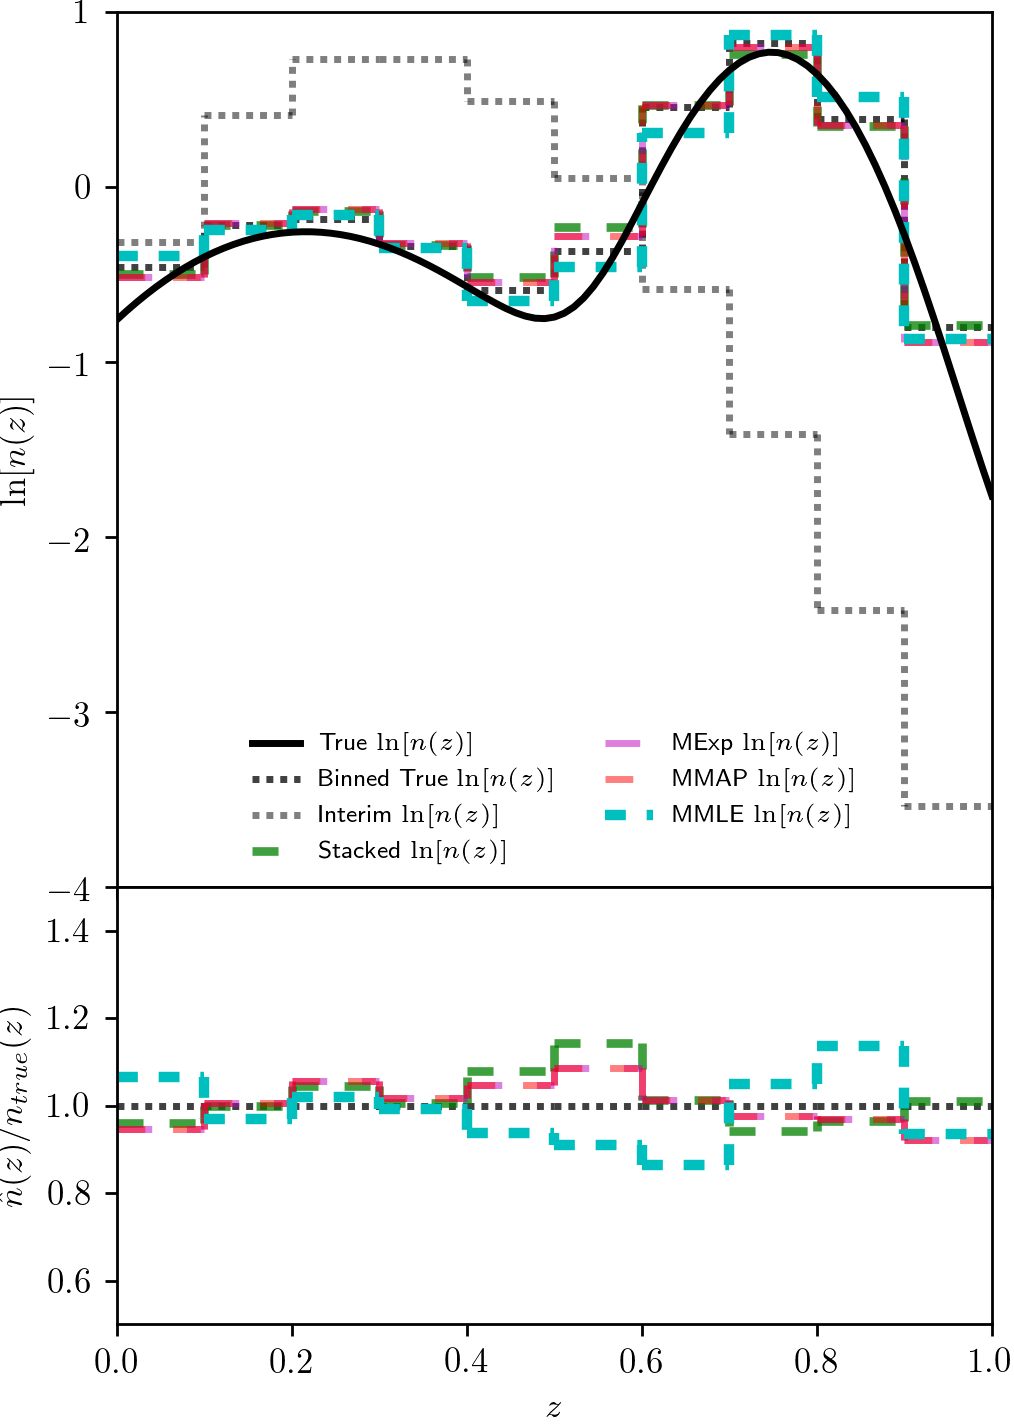
\includegraphics[width=0.5\textwidth]{fig/training_prior/estimators.png}	
		\caption{[The case of a low-$z$ favoring interim prior was a very compelling test in the previous version but somehow isn't anymore.]}
		\label{fig:trainintpr}
	\end{center}
\end{figure}

\section{Application to Realistic Mock Data}
\label{sec:application}

To show how the choice of $n(z)$ estimator propagates to cosmological constraints, we apply \chippr to a data from a realistic cosmological simulation (probably \texttt{Buzzard}) with photo-$z$ PDFs produced by a popular method (probably \texttt{BPZ}).

\subsection{Mock Data \& Metrics}
\label{sec:appintro}

As in Sec. \ref{sec:validintro}, the mock data takes the form of photo-$z$ interim posteriors, but that is where the similarity ends.  These photo-$z$ interim posteriors are derived from the photometry resulting from the \texttt{Buzzard} simulation by way of \texttt{BPZ}.  Because the simulation begins with setting true values of the cosmological parameters, we can propagate the different estimators of $n(z)$ through a forecasting code (which one?) to generate error ellipses on the cosmological parameters.

\subsubsection{Mock Data}
\label{sec:buzzard}

We summarize the details of the \texttt{Buzzard} simulation here.

\subsubsection{Cosmological Constraint Metric}
\label{sec:cosmo}

Because the realistic mock data of Sec. \ref{sec:buzzard} is associated with true values of the cosmological parameters, we may compare the quality of cosmological constraints under different estimators of $n(z)$, creating a figure like Fig. \ref{fig:scgsr}.  We perform this analysis using a forecasting code that takes $n(z)$ and produces projected error ellipses in the space of cosmological parameters.  

\begin{figure}
	\begin{center}
		Not my figure! (N. MacCrann via J. DeRose)
		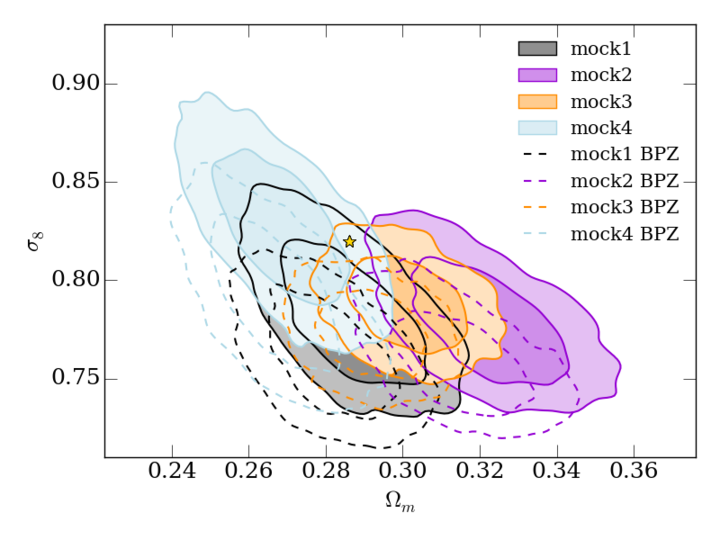
\includegraphics[width=0.5\textwidth]{cosmo_constraints.png}
		\caption{[I'd like to be able to make a plot like this with the different $n(z)$ estimators produced by \texttt{chippr} from the same set of photo-$z$ PDFs.  Then I can calculate some metrics of the accuracy and precision of the error distributions relative to the true values of the cosmological parameters that produced the mock data.]}
		\label{fig:scgsr}
	\end{center}
\end{figure}

% \textbf{Check Dark Energy Task Force metrics on error ellipses, multi-dimensional KLD, centroid offset, etc.}

\subsection{Results}
\label{sec:results}

\begin{figure}
	\begin{center}
% 		\includegraphics[width=0.5\textwidth]{money.png}
		\caption{[moneyplot of error ellipses resulting from different $n(z)$ estimators]}
		\label{fig:money}
	\end{center}
\end{figure}

\section{Discussion}
\label{sec:discussion}

The results of Fig \ref{fig:money} have significant implications for the developing data analysis pipelines of next-generation telescope surveys.  However, the method presented here has its own limitations, which are reiterated to discourage the community from applying this work inappropriately.

We intend to pursue a number of extensions of the work presented in this paper in future work.

\section{Conclusion}
\label{sec:conclusion}

We now summarize answers to the questions posed in the introduction:

\begin{itemize}
	\item Existing $n(z)$ estimation methods produce biased estimators that propagate to inaccuracies in characterizing the cosmological parameters.
	\item Photo-$z$ PDFs are probabilistic data products so must be handled in a mathematically consistent manner such as the probabilistic graphical model outlined in this paper.
	\item In addition to coming with its own error distribution, the $n(z)$ estimator produced by \chippr is quantifiably more accurate than established estimators.
	\item Propagation of the \chippr result leads to a quantifiable improvement in the constraints on cosmological parameters.
\end{itemize}

In conclusion, we discourage the community from continuing to use the stacked estimator and reductions of photo-$z$ PDFs to redshift point estimates in obtaining estimators of $n(z)$.  \chippr is freely available to the community for incorporation into evolving data analysis pipelines.  

%\section{Introduction}
%\label{sec:introduction}
%
%The redshift distribution $n(z)$ is necessary for calculating two-point statistics of galaxy properties used to determine the cosmological parameter values that inform our understanding of the evolution of large-scale structure in the universe \citep{masters_mapping_2015}.  Inaccurate estimates of $n(z)$ can significantly impact the constraining power of a galaxy survey, biasing recovery of the cosmological parameters.  For example, if the $n(z)$ used in analysis is offset from the true $n(z)$ by a small, negative constant, it results in underestimating $w_{0}$ and overestimating $\sigma_{8}$ \citep{samuroff_simultaneous_2017}.
%
%Though the redshift density function has traditionally been determined from spectroscopically observed redshifts, modern galaxy surveys including DES, LSST, Euclid, and WFIRST seek to obtain two-point statistics of redshift from samples of galaxies for which spectroscopic redshifts are unavailable, either due to their large numbers or their low brightnesses.  For decades, photometrically estimated redshifts (photo-$z$s) have been the leading alternative to spectroscopically observed redshifts, though they suffer from issues of precision in the form of an intrinsic scatter and accuracy in the form of catastrophic outliers, as well as other systematics imparted by the properties of the survey, data reduction pipeline(s), and assumptions underlying the analysis \citep{baum_photoelectric_1962}.  These weaknesses are illuminated by a probabilistic interpretation of photo-$zs$; if these nontrivial uncertainties were expressed as a probability distribution function (PDF) over redshift, photo-$z$s could be replaced by photo-$z$ PDFs containing more information than a simple point estimate \citep{koo_overview_1999}.  Such data products have been commonly released by photometric galaxy surveys since SDSS DR7 \citep{abazajian_seventh_2009} using a great variety of methods.
%
%Methods for using photo-$z$ PDFs in cosmological inference remain underdeveloped, with many survey pipelines reducing them to familiar point estimators that are compatible with existing technology or engaging with them heuristically in a manner inconsistent with their probabilistic nature.  Stacking photo-$z$ PDFs, or other mathematically equivalent methods, to obtain an estimator of $n(z)$ is especially popular \citep{cunha_estimating_2009, sheldon_photometric_2012}.  However, photo-$z$ PDFs are probabilistic data products that must be handled in a fully consistent, probabilistic manner; hierarchical inference is the only mathematically valid way to do inference with photo-$z$ PDFs and other probabilistic quantities.
%
%It is desirable to create rigorous methods for using photo-$z$ PDFs in inference, beginning with the simplest one-point statistic of redshift, $n(z)$.  In the spirit of \citet{hogg_inferring_2010, foreman-mackey_exoplanet_2014}, this paper derives a mathematically rigorous approach to inferring $n(z)$ in Sec. \ref{sec:method}.  The presentation of a public code implementing this novel technique is given in Sec. \ref{sec:model_specifics}.  The code is validated on mock data and tested on a subset of BOSS DR10 data in Sec. \ref{sec:experiments}.  We conclude and discuss future directions in Sec. \ref{sec:discussion}.
%
%\section{Method}
%\label{sec:method}
%
%The redshift distribution $n(z)$ may be understood as the probability of finding a galaxy at a redshift $z$.  We may express $n(z)$ in terms of some functional form $f_{\vec{\theta}}(z)$ with parameters comprising $\vec{\theta}$ according to Eq. \ref{eq:parametrization}.  
%\begin{align}
%\label{eq:parametrization}
%n(z) &\equiv f_{\vec{\theta}}(z)\ \equiv\ p(z|\vec{\theta})
%\end{align}
%In this work, we wish to characterize the posterior distribution $p(\vec{\theta}|\textul{D})$ of the parameters contained in $\vec{\theta}$ defining $n(z)$ given all available data $\textul{D}$.  The likelihood $p(z|\vec{\theta})$ represents the probability of a random variable, in this case redshift $z$, given the parameters in $\vec{\theta}$ defining the distribution $n(z)$ from which it is drawn.  Our model for inferring $p(\vec{\theta}|\textul{D})$ will be introduced in Sec. \ref{sec:derivation}, and alternative methods of estimating $\vec{\theta}$ will be presented in Sec. \ref{sec:alternatives}.
%
%\subsection{Derivation}
%\label{sec:derivation}
%
%Inference of $p(\vec{\theta}|\textul{D})$ is perfectly suited to a hierarchical Bayesian model.  In this problem, the available data $\textul{D}$ is a catalog of photometry $\{\vec{d}_{i}\}$ of individual galaxies $i$ where each $\vec{d}_{i}$ is a random variable that is a function of its redshift parameter $z_{i}$; the redshift parameters $\{z_{i}\}$ are independently drawn from a function defined by hyperparameters in $\vec{\theta}$.  These physical relationships may be illustrated in Fig. \ref{fig:pgm} by a directed acyclic graph representing a probabilistic graphical model (PGM).
%\begin{figure}
%\begin{center}
%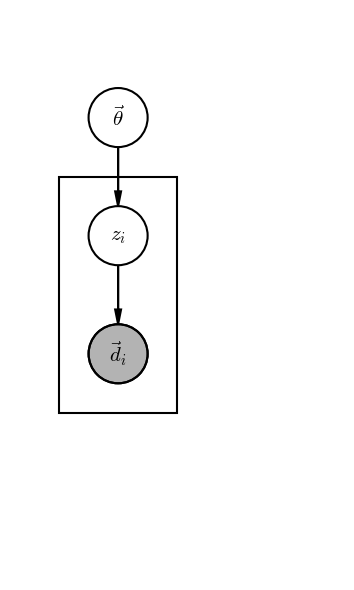
\includegraphics[width=0.5\textwidth]{pgm.png}
%\caption{This directed acyclic graph corresponds to a PGM for a hierarchical inference of $p(\vec{\theta}|\{\vec{d}_{i}\})$.  In this graph, all random variables are shown in circles, with observed variables shown in shaded circles.  Relationships between variables are indicated by arrows.  The box indicates that there are a number of copies of the relationships between boxed parameters, each independent of all others.  The hyperparameters $\vec{\theta}$ representing $n(z)$ are at the top.  Independently drawn from a function of the hyperparameters $\vec{\theta}$ are galaxy redshifts $\{z_{i}\}$ below.  The observed galaxy photometry $\{\vec{d}_{i}\}$, shown in shaded circles, is determined by the redshifts above.}
%\label{fig:pgm}
%\end{center}
%\end{figure}
%This PGM may be used as the basis for a derivation of the desired hyperposterior $p(\vec{\theta}|\{\vec{d}_{i}\})$, assuming our physical model is complete.  From this point on, we will work solely with log probabilities.
%
%We begin with Eq. \ref{eq:hyperbayes} by applying Bayes' Rule to express the log-hyperposterior $\ln\left[p(\vec{\theta}|\{\vec{d}_{i}\})\right]$ in terms of the log-hyperlikelihood $\ln\left[p(\{\vec{d}_{i}\}|\vec{\theta})\right]$.
%\begin{align}
%\label{eq:hyperbayes}
%\ln\left[p(\vec{\theta}|\{\vec{d}_{i}\})\right] &\propto \ln\left[p(\vec{\theta})\right] + \ln\left[p(\{\vec{d}_{i}\}|\vec{\theta})\right]
%\end{align}
%To do this, we will choose a log-hyperprior distribution $\ln\left[p(\vec{\theta})\right]$ representing our beliefs about the distribution of the hyperparameters $\vec{\theta}$ in terms of fixed variables that we will assume are known.
%
%The log-hyperlikelihood $\ln\left[p(\{\vec{d}_{i}\}|\vec{\theta})\right]$ contains no explicit reference to redshifts, therefore, we employ the PGM to write the marginalization over the redshifts in Eq. \ref{eq:marginalization}.
%\begin{align}
%\label{eq:marginalization}
%\ln\left[p(\{\vec{d}_{i}\}|\vec{\theta})\right] &= \ln\left[\int\ p(\{\vec{d}_{i}\}|\{z_{i}\})\ p(\{z_{i}\}|\vec{\theta})\ d\{z_{i}\}\right]
%\end{align}
%We shall handle the two terms in the integral separately.
%
%The first term is the likelihood of all galaxy photometry given all galaxy redshifts.  If we assume independence of galaxy photometry, such that $p(\vec{d}_{i}|\{\vec{d}_{i'\neq i}\}, \{z_{i}\})=p(\vec{d}_{i}|z_{i})$, then we may write Eq. \ref{eq:independentdata}.
%\begin{align}
%\label{eq:independentdata}
%\ln\left[p(\{\vec{d}_{i}\}|\{z_{i}\})\right] &= \sum_{i}\ln\left[p(\vec{d}_{i}|z_{i})\right]
%\end{align}
%The second term may also be expanded as in Eq. \ref{eq:independentredshifts} by assuming that all galaxy redshifts are drawn independently from $n(z)$.
%\begin{align}
%\label{eq:independentredshifts}
%\ln\left[p(\{z_{i}\}|\vec{\theta})\right] &= \sum_{i}\ln\left[p(z_{i}|\vec{\theta})\right]
%\end{align}
%Since all galaxy redshifts are independent of one another, an integral over the aggregate $\int\dots d\{z_{i}\}$ is simply the product of the integrals over each one $\prod_{i}\int\dots dz_{i}$.  Thus, the log-hyperlikelihood can be written according to Eq. \ref{eq:log-hyperlikelihood}.
%\begin{align}
%\label{eq:log-hyperlikelihood}
%\ln\left[p(\{\vec{d}_{i}\}|\vec{\theta})\right] &= \sum_{i}\ln\left[\int\ p(\vec{d}_{i}|z_{i})\ p(z_{i}|\vec{\theta})\ dz_{i}\right]
%\end{align}
%The expression of Eq. \ref{eq:log-hyperlikelihood} contains two types of quantities.  The $\{p(z_{i}|\vec{\theta})\}$ are known likelihoods that will be equal to $\{f_{\vec{\theta}}(z_{i})\}$.  The $\{p(\vec{d}_{i}|z_{i})\}$, however, are likelihoods that are unknown and in general unknowable, and it is worth discussing these facts.  
%
%Photo-$z$ PDFs are commonly written simply as $p(z)$, but this notation oversimplifies their substance.  Whether determined by way of template-fitting or machine learning, photo-$z$ PDFs are dependent on the data $\vec{d}$ from which they are calculated.  This data $\vec{d}$ must be considered to be a quantity upon which the redshift $z$ is conditioned, otherwise normalizing a photo-$z$ PDF would require integrating over all possible values of $\vec{d}$.  This means that photo-$z$ PDFs are posteriors, probabilities of parameters $z$ conditioned on data $\vec{d}$.  However, where there is a posterior, there is always a prior.  Photo-$z$ PDFs are in general \textit{interim} posteriors, because in addition to being conditioned on observations, they are also conditioned on an interim prior in the form of a particular value $\vec{\theta}^{*}$ of $\vec{\theta}$ necessary for computing the photo-$z$ PDF.  In the case of template-fitting methods, the interim prior is usually specified as an input to the photo-$z$ PDF production code, and it often takes the form of an initial guess for $\vec{\theta}$ based on the results of previous galaxy surveys or simulations thereof; in the case of machine learning methods, the interim prior may be explicitly derived from the training set or implicitly produced in the process of determining the photo-$z$ PDFs, and the interim prior is not always revealed to the user.   Hierarchical inference may be performed only when the interim prior is known, which means it will only be possible for photo-$z$ PDFs made via certain methods.
%
%Since the data products from which we hope to probe the log-hyperposterior are themselves posteriors, we must express the likelihoods $\{p(\vec{d}_{i}|z_{i})\}$ of Eq. \ref{eq:log-hyperlikelihood} in terms of the photo-$z$ PDFs $\{p(z_{i}|\vec{d}_{i}, \vec{\theta}^{*})\}$.  We start by multiplying the likelihood by an inspired factor of unity written in terms of the photo-$z$ interim posterior we have at hand, as in Eq. \ref{eq:unity}.
%\begin{align}
%\label{eq:unity}
%p(\vec{d}_{i}|z_{i}) &= p(\vec{d}_{i}|z_{i})\ \frac{p(z_{i}|\vec{d}_{i}, \vec{\theta}^{*})}{p(z_{i}|\vec{d}_{i}, \vec{\theta}^{*})}
%\end{align}
%Next, we expand the denominator in terms of Bayes' Rule to obtain Eq. \ref{eq:bayes}.
%\begin{align}
%\label{eq:bayes}
%p(\vec{d}_{i}|z_{i}) &= p(\vec{d}_{i}|z_{i})\ p(z_{i}|\vec{d}_{i}, \vec{\theta}^{*})\ \frac{p(\vec{d}_{i}|\vec{\theta}^{*})}{p(z_{i}|\vec{\theta}^{*})\ p(\vec{d}_{i}|z_{i}, \vec{\theta}^{*})}
%\end{align}
%Because the redshift $z_{i}$ is independent of the interim prior $\vec{\theta}^{*}$, the interim likelihood $p(\vec{d}_{i}|z_{i}, \vec{\theta}^{*})$ may be expanded further as in Eq. \ref{eq:expansion}.
%\begin{align}
%\label{eq:expansion}
%p(\vec{d}_{i}|z_{i}) &= p(\vec{d}_{i}|z_{i})\ p(z_{i}|\vec{d}_{i}, \vec{\theta}^{*})\ \frac{p(\vec{d}_{i}|\vec{\theta}^{*})}{p(z_{i}|\vec{\theta}^{*})\ p(\vec{d}_{i}|z_{i})\ p(\vec{d}_{i}|\vec{\theta}^{*})}
%\end{align}
%We cancel the terms $p(\vec{d}_{i}|z_{i})$ and $p(\vec{d}_{i}|\vec{\theta}^{*})$ that appear in both the numerator and denominator of Eq. \ref{eq:expansion} to obtain Eq. \ref{eq:cancellation}.
%\begin{align}
%\label{eq:cancellation}
%p(\vec{d}_{i}|z_{i}) &= \frac{p(z_{i}|\vec{d}_{i}, \vec{\theta}^{*})}{p(z_{i}|\vec{\theta}^{*})}
%\end{align}
%
%Finally we may return to Eq. \ref{eq:hyperbayes} to express the log-hyperposterior $\ln\left[p(\vec{\theta}|\{\vec{d}_{i}\})\right]$ in terms of the photo-$z$ interim posteriors $\{p(z_{i}|\vec{d}_{i}, \vec{\theta}^{*})\}$, as in Eq. \ref{eq:final}.
%\begin{align}
%\label{eq:final}
%\ln\left[p(\vec{\theta}|\{\vec{d}_{i}\})\right] &\propto \ln\left[p(\vec{\theta})\right] + \sum_{i}\ln\left[\int\ p(z_{i}|\vec{d}_{i}, \vec{\theta}^{*})\ \frac{p(z_{i}|\vec{\theta})}{p(z_{i}|\vec{\theta}^{*})}\ dz_{i}\right]
%\end{align}
%Now we have an expression for a quantity proportional to the log-hyperposterior we desire!  Though the constant of proportionality, $p(\{\vec{d}_{i}\})$ is in general not possible to calculate, we may still characterize the log-hyperposterior by way of MCMC sampling and optimization, which will be discussed in Sec. \ref{sec:implementation}.
%
%Several assumptions were noted in the above derivation; for clarity, they will be enumerated below, where their limitations will be discussed.
%\begin{enumerate}
%\item The PGM is an expression of our beliefs about the physics of the problem, and the inference will only be valid to the degree that the model is correct.  One can easily think of ways in which the PGM of Fig. \ref{fig:pgm} is incomplete; for example, intrinsic galaxy SEDs will evolve with redshift.  However, we assume that physical processes not represented in the PGM of Fig. \ref{fig:pgm} are subdominant and may thus be neglected.
%\item We must choose a hyperprior $p(\vec{\theta})$; we assume that our choice of a sufficiently general hyperprior that will not be a dominant source of information in the hyperposterior is successful.  If we choose poorly, the hyperprior may dominate over the hyperlikelihood, downweighting the significance of the data in determining the hyperposterior or biasing the result based on a misunderstanding of the underlying physics.
%\item We assume independence of galaxies in our catalog such that each galaxy's photometry $\vec{d}_{i}$ is independent from all other galaxies' photometry $\{\vec{d}_{i'\neq i}\}$ and all other galaxies' redshifts $\{z_{i'\neq i}\}$.  However, the photometry $\{\vec{d}_{i}\}$ will inherently share instrumental and systematic effects due to being observed with the same telescope as part of a single survey project.  Furthermore, there may be blended objects or other correlations between the redshifts of different galaxies.  We must assume that such effects are negligible and will not consider them in this treatment.  
%\item We assume that the interim prior is known to us, either as input to or output of the method producing the photo-$z$ interim posteriors.  Furthermore, it must be representable in the parametrization of $f_{\vec{\theta}}(z)$, i.e. our model $f_{\vec{\theta}}(z)$ for $n(z)$ must be flexible enough to encompass both the true distribution we aim to probe and the interim prior.
%\item Finally, we assume that the photo-$z$ interim posteriors $\{p(z_{i}|\vec{d}_{i}, \vec{\theta}^{*})\}$ are accurate.  There is some evidence that photo-$z$ PDFs derived by different methods disagree with one another or are strongly dependent on the interim prior.  However, the choice of the technique by which the photo-$z$ interim posteriors are determined is outside the scope of this paper.
%\end{enumerate}
%
%\subsection{Alternative methods}
%\label{sec:alternatives}
%
%This method is presented in contrast to existing methods for inferring $n(z)$ from photo-$z$ PDFs, which fall into two broad categories: stacking and point estimation.  Stacking assumes Eq. \ref{eq:stacking}, where the constant of proportionality is chosen to ensure $\int f_{\vec{\theta}}(z)\ dz$ is unity.
%\begin{align}
%\label{eq:stacking}
%f_{\vec{\theta}}(z) &\propto \sum_{i}p(z_{i}|\vec{d}_{i}, \vec{\theta}^{*})
%\end{align}
%
%\section{Implementation}
%\label{sec:implementation}
%
%We introduce the Cosmological Hierarchical Inference with Probabilistic Photometric Redshifts (CHIPPR) code as a comprehensive package for estimating $n(z)$ from catalogs of photo-$z$ PDFs.  In particular, CHIPPR implements both sampling and optimization of Eq. \ref{eq:final} and compares the results to those of the more traditional approaches presented in Sec. \ref{sec:alternatives}.
%
%\section{Experiments}
%\label{sec:experiments}
%
%\section{Discussion}
%\label{sec:discussion}

%\appendix{}

\begin{acknowledgements}
AIM thanks Mohammadjavad Vakili for insightful input on statistics, Geoffrey Ryan for assistance in debugging, and Boris Leistedt for helpful comments provided in the preparation of this paper.
\end{acknowledgements}

%\bibliographystyle{apj}
%\bibliography{references}

\end{document}
